% TI Agent: journal-style paper (Elsevier elsarticle, numbered references)
% Build:  latexmk -pdf paper.tex      (pdflatex + bibtex)
% Shares figures and bibliography with the project report in ../report/.

\documentclass[preprint,11pt]{elsarticle}

\usepackage[T1]{fontenc}
\usepackage[utf8]{inputenc}
\usepackage{lmodern}
\usepackage{microtype}
\usepackage[margin=2.5cm]{geometry}
\usepackage{amsmath, amssymb}
\usepackage{graphicx}
\usepackage{booktabs}
\usepackage{tabularx}
\usepackage{xcolor}
\usepackage{tikz}
\usetikzlibrary{positioning, arrows.meta, shapes.geometric, fit, backgrounds, calc}
\usepackage{pgfplots}
\pgfplotsset{compat=1.18}
\usepackage{lineno}
\usepackage[colorlinks=true, linkcolor=blue!50!black, citecolor=blue!50!black, urlcolor=blue!50!black]{hyperref}
\graphicspath{{../report/figures/}}

\definecolor{accent}{HTML}{1F5FA8}
\definecolor{ink}{HTML}{22262B}
\definecolor{muted}{HTML}{6B7280}
\definecolor{boxfill}{HTML}{EEF3FA}
\definecolor{storefill}{HTML}{E8F3EC}
\definecolor{extfill}{HTML}{F5F1E8}
\definecolor{warnfill}{HTML}{FBEDEA}
\definecolor{good}{HTML}{2E7D4F}
\definecolor{bad}{HTML}{B23B3B}
\definecolor{neutral}{HTML}{8A8F98}

\tikzset{
  block/.style   = {draw=accent!70, fill=boxfill, rounded corners=2pt, align=center, font=\footnotesize,
                    minimum height=8mm, inner sep=3pt, text width=#1,
                    execute at begin node={\hyphenpenalty=10000\exhyphenpenalty=10000}},
  block/.default = 2.6cm,
  ext/.style     = {draw=muted!70, fill=extfill, rounded corners=2pt, align=center, font=\footnotesize,
                    minimum height=7mm, inner sep=3pt, text width=#1,
                    execute at begin node={\hyphenpenalty=10000\exhyphenpenalty=10000}},
  ext/.default   = 2.4cm,
  store/.style   = {cylinder, shape border rotate=90, aspect=0.22, draw=good!70, fill=storefill,
                    align=center, font=\footnotesize, minimum height=13mm, text width=#1},
  store/.default = 2.6cm,
  arr/.style     = {-{Stealth[length=2mm]}, thick, draw=ink!70},
  dasharr/.style = {-{Stealth[length=2mm]}, thick, dashed, draw=muted},
  lbl/.style     = {font=\scriptsize, text=muted, align=center},
  group/.style   = {draw=muted!50, dashed, rounded corners=4pt, inner sep=6pt},
}
\newcommand{\code}[1]{\texttt{#1}}

\journal{a peer-reviewed journal (to be chosen)}

\begin{document}

\begin{frontmatter}

\title{Grounded, point-in-time equity research with a small local language model:\\
design and first deployment of TI Agent}

\author{Nanda Srikanth Saroj Kumar Nanda}
\address{Independent researcher}

\begin{abstract}
Large language models (LLMs) are attractive for equity research because most of an analyst's work is
reading, yet two habits make them hazardous in finance: they produce unsupported numbers, and they leak
information from after the date they are asked to reason about. We present TI Agent, a system that lets a
small open-weight model (Qwen3.5, 4B parameters, run locally) write medium- and long-horizon views on US
equities while the surrounding code removes both hazards. All inputs carry the time at which they became
public and are filtered to an as-of date; a two-stage pipeline screens the S\&P 500 and S\&P MidCap 400 on
quality and momentum and spends retrieval and generation only on the top twenty; hybrid retrieval with
reciprocal rank fusion and cross-encoder reranking supplies citable passages; and a tool-using agent may
save a view only if every citation was retrieved in the same session and every number matches a value a
tool computed. Results are published as a password-encrypted static file, so the system needs no server.
In its first deployment on consumer hardware the agent produced 40 views for 20 stocks in 32 minutes,
containing 470 numeric claims and 3.8 citations per view on average, all of which passed the checks.
To get there, the guardrails rejected 49 of 89 save attempts, 26 of them for numbers that no tool had
returned. Reranking raised the share of on-topic retrieval results on a ten-query test set from 7 to 10.
We describe the design, report these measurements, and pre-specify the protocol for evaluating the views
against realised returns.
\end{abstract}

\begin{keyword}
large language models \sep retrieval-augmented generation \sep look-ahead bias \sep
financial NLP \sep tool-using agents \sep grounded generation
\end{keyword}

\end{frontmatter}

\linenumbers

% ==================================================================
\section{Introduction}
\label{sec:intro}

Before an analyst forms a view on a company, most of the work is reading: annual and quarterly reports,
news, and the numbers behind the price chart. Large language models read quickly and summarise well, and
retrieval-augmented generation (RAG) lets them draw on documents they were never trained on
\cite{lewis2020retrievalaugmented, gao2023retrievalaugmented}. Two properties nevertheless make them risky
for financial analysis.

The first is unsupported numbers. A fluent model will state a growth rate or a margin with the same
confidence whether the figure came from a document or from nowhere. The second is look-ahead bias. A model
asked about a past date may use what it memorised during training about later events; Glasserman and Lin
show that sentiment extracted with GPT models already carries such bias \cite{glasserman2023assessing}.
Domain-specific models such as BloombergGPT \cite{wu2023bloomberggpt} and FinGPT \cite{yang2023fingpt}
improve financial language understanding but do not remove either problem, and they are expensive to run.

This paper asks a practical question: \emph{how far can a small, free, locally run model go if the system
around it is responsible for correctness?} We describe TI Agent, which runs end to end on a single laptop
with free data sources and publishes its output without a server. Its contributions are:

\begin{enumerate}
  \item A point-in-time data layer in which every price, filing, financial fact and macro observation keeps
        the moment it became public, so that every read can be restricted to an as-of date, including inside
        the vector-search functions (Section~\ref{sec:data}).
  \item A two-stage universe design that screens roughly 900 stocks cheaply on quality and momentum and
        spends retrieval and generation only on the top twenty (Section~\ref{sec:screen}).
  \item Code-enforced guardrails for a tool-using agent: fixed ticker and date, citations that must have
        been retrieved in the same session, and numbers that must match tool outputs
        (Section~\ref{sec:agent}).
  \item A serverless delivery method that publishes results as one authenticated-encrypted file decrypted
        in the reader's browser (Section~\ref{sec:delivery}).
  \item Measurements from the first full deployment, and a pre-specified protocol for evaluating the
        views against realised returns (Sections~\ref{sec:results} and \ref{sec:protocol}).
\end{enumerate}

We make no claim that the views have predictive value; that question requires outcome data that does not
exist yet, and Section~\ref{sec:protocol} defines how it will be answered.

% ==================================================================
\section{Related work}
\label{sec:related}

\paragraph{Retrieval-augmented generation} RAG conditions generation on retrieved passages
\cite{lewis2020retrievalaugmented}; Gao et al.\ survey the many variants \cite{gao2023retrievalaugmented}.
Dense retrievers such as DPR \cite{karpukhin2020dense} and Sentence-BERT \cite{reimers2019sentencebert}
capture meaning, while lexical retrieval remains a strong baseline on out-of-domain text \cite{thakur2021beir}.
Reciprocal rank fusion combines ranked lists without tuning \cite{cormack2009rrf}, and cross-encoder rerankers
trained on MS MARCO improve precision at the top of the list \cite{nogueira2019passage, bajaj2016marco}.
Liu et al.\ show that models under-use information placed in the middle of long contexts \cite{liu2023lost},
which argues for short, diverse contexts.

\paragraph{Grounding and citations} Gao et al.\ benchmark LLMs that generate text with citations and find
citation quality to be a weak point \cite{gao2023enabling}. Our approach is complementary: rather than
measuring citation quality after the fact, the system refuses to store a view whose citations or numbers
cannot be traced to the session's tool outputs.

\paragraph{Tool-using agents} ReAct interleaves reasoning with actions \cite{yao2022react}, and Toolformer
shows that models can learn when to call tools \cite{schick2023toolformer}. We use a ReAct-style loop with a
small model from the Qwen3 family \cite{yang2025qwen3}.

\paragraph{Financial NLP and look-ahead bias} The FinBERT model \cite{araci2019finbert} provides domain
sentiment at low cost; BloombergGPT \cite{wu2023bloomberggpt} and FinGPT \cite{yang2023fingpt} pursue general financial LLMs.
Glasserman and Lin quantify look-ahead bias in LLM-based return prediction \cite{glasserman2023assessing}.
Our data layer addresses the part of the problem the system controls, namely the inputs.

\paragraph{Factor screens} The screen combines the momentum effect \cite{jegadeesh1993returns} with a
profitability filter in the spirit of the quality literature \cite{novymarx2013other}.

% ==================================================================
\section{System design}
\label{sec:design}

Figure~\ref{fig:arch} gives an overview. Modules communicate only through a PostgreSQL database with the
\code{pgvector} extension; every read and write passes through one store interface, which the test suite
replaces with an in-memory fake (130 offline tests).

\begin{figure}[t]
\centering
\resizebox{\linewidth}{!}{%
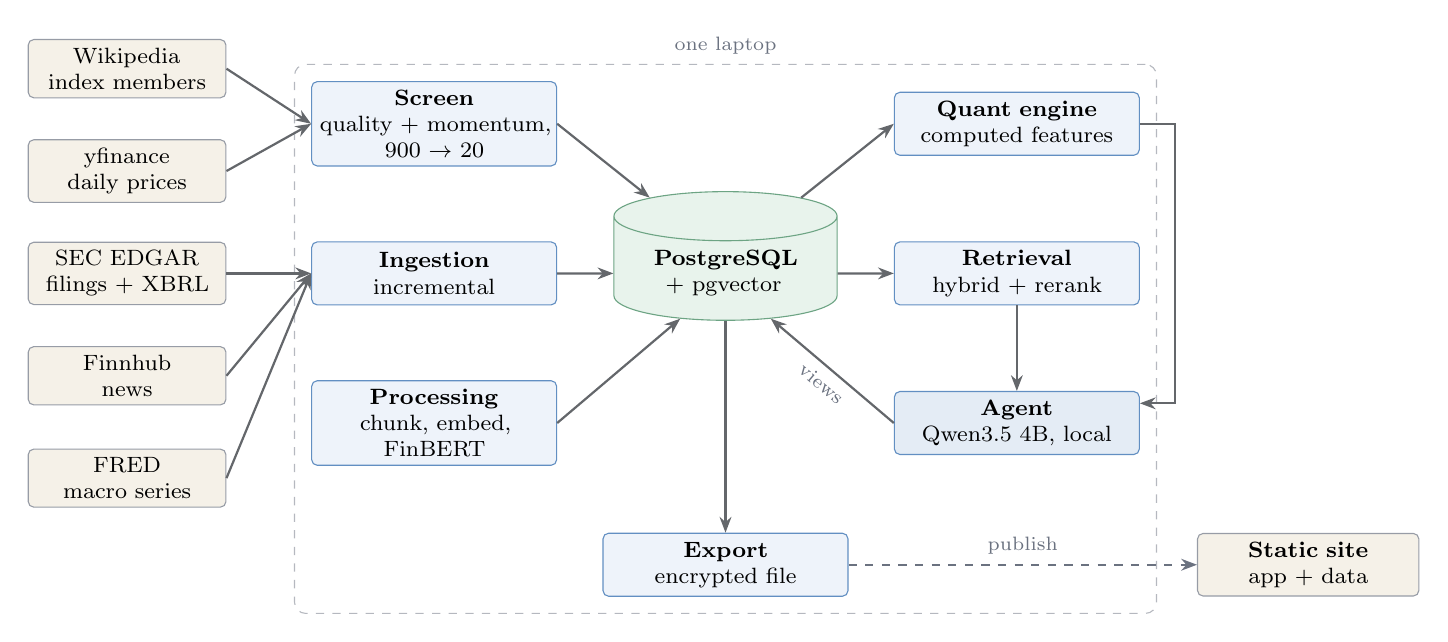
\begin{tikzpicture}
  \node[ext=2.3cm] (wiki) at (0, 2.6)  {Wikipedia\\index members};
  \node[ext=2.3cm] (yf)   at (0, 1.3)  {yfinance\\daily prices};
  \node[ext=2.3cm] (sec)  at (0, 0)    {SEC EDGAR\\filings + XBRL};
  \node[ext=2.3cm] (fin)  at (0, -1.3) {Finnhub\\news};
  \node[ext=2.3cm] (fred) at (0, -2.6) {FRED\\macro series};
  \node[block=2.9cm] (screen) at (3.9, 1.9)  {\textbf{Screen}\\quality + momentum, 900 $\to$ 20};
  \node[block=2.9cm] (ingest) at (3.9, 0)    {\textbf{Ingestion}\\incremental};
  \node[block=2.9cm] (proc)   at (3.9, -1.9) {\textbf{Processing}\\chunk, embed, FinBERT};
  \node[store=2.6cm] (db)     at (7.6, 0)    {\textbf{PostgreSQL}\\+ pgvector};
  \node[block=2.9cm] (quant)  at (11.3, 1.9) {\textbf{Quant engine}\\computed features};
  \node[block=2.9cm] (ret)    at (11.3, 0)   {\textbf{Retrieval}\\hybrid + rerank};
  \node[block=2.9cm, fill=accent!12] (agent) at (11.3, -1.9) {\textbf{Agent}\\Qwen3.5 4B, local};
  \node[block=2.9cm] (export) at (7.6, -3.7) {\textbf{Export}\\encrypted file};
  \node[ext=2.6cm] (pages) at (15.0, -3.7) {\textbf{Static site}\\app + data};
  \begin{scope}[on background layer]
    \node[group, fit=(screen)(proc)(db)(quant)(agent)(export), label={[lbl]above:one laptop}] {};
  \end{scope}
  \draw[arr] (wiki.east) -- (screen.west);
  \draw[arr] (yf.east) -- (screen.west);
  \draw[arr] (sec.east) -- (ingest.west);
  \draw[arr] (fin.east) -- (ingest.west);
  \draw[arr] (fred.east) -- (ingest.west);
  \draw[arr] (screen.east) -- (db.north west);
  \draw[arr] (ingest) -- (db);
  \draw[arr] (proc.east) -- (db.south west);
  \draw[arr] (db.north east) -- (quant.west);
  \draw[arr] (db.east) -- (ret.west);
  \draw[arr] (quant.east) -- ++(0.45,0) |- ([yshift=2.5mm]agent.east);
  \draw[arr] (ret) -- (agent);
  \draw[arr] (agent.west) -- node[lbl, below, sloped]{views} (db.south east);
  \draw[arr] (db.south) -- (export.north);
  \draw[dasharr] (export.east) -- node[lbl, above]{publish} (pages.west);
\end{tikzpicture}}
\caption{Architecture. Everything inside the dashed box runs on one consumer laptop.}
\label{fig:arch}
\end{figure}

\subsection{Point-in-time data layer}
\label{sec:data}

Five free sources supply daily prices (yfinance), company news (Finnhub), the text of 10-K, 10-Q and 8-K
filings (SEC EDGAR), every financial fact as reported in each filing (SEC XBRL) and eight macro series
(FRED). Table~\ref{tab:pit} lists the timestamp that defines when each item became public. Every read
filters on an as-of date $t$; for retrieval the filter lives inside the SQL search functions and is checked
again in application code, and a regression test plants a document dated after $t$ and asserts that it is
never returned.

\begin{table}[t]
\centering\small
\caption{Timestamps that define public availability, and the corresponding read rule for an as-of date $t$.}
\label{tab:pit}
\begin{tabular}{@{}lll@{}}
\toprule
Data & Timestamp & Read rule \\
\midrule
Prices & trading date & $\text{date} < t$ \\
News & publication time & $\text{published} < t$ \\
Filings & SEC acceptance time & $\text{published} < t$ \\
XBRL facts & filing date of each fact & $\text{filed} < t$; latest filing wins \\
Macro series & observation date $+$ release lag $\ell$ & $\text{date} + \ell \le t$ \\
\bottomrule
\end{tabular}
\end{table}

Text is split at sentence boundaries into chunks of at most 180 words with 30 words of overlap, embedded
with MiniLM \cite{wang2020minilm} (384 dimensions) and indexed with HNSW \cite{malkov2016efficient}; a
full-text index supports keyword search. Because HNSW applies filters after the index scan, ticker-filtered
queries use an exact scan to avoid silently returning fewer results. News items are scored with FinBERT
\cite{araci2019finbert}.

After an initial two-year backfill, ingestion is incremental. Adjusted prices are re-based after dividends
and splits, so each incremental download overlaps the last stored week and a ticker is re-downloaded in full
when its last stored adjusted close disagrees with the new one. A retention step deletes rows older than the
longest look-back of any reader (e.g.\ 800 days of prices), but never a passage that some view cites.

\subsection{Quantitative features}

All numbers the agent may use come from deterministic functions over the stored data: trailing returns,
moving averages, RSI \cite{wilder1978new}, MACD, volatility, drawdown, beta and relative strength against
SPY; point-in-time fundamentals rebuilt from as-reported XBRL facts (trailing-twelve-month revenue, margins,
free cash flow, P/E, leverage); news-sentiment aggregates; and a macro snapshot with release lags.

\subsection{Two-stage universe}
\label{sec:screen}

Running retrieval and generation on the full S\&P 500 and S\&P MidCap 400 would exceed ten GPU-hours per
week on our hardware. The first stage therefore screens all members using prices and SEC data only. A
company passes the quality filter if its latest fiscal quarter ended less than 200 days before $t$ and its
trailing net margin and free cash flow are positive. Among those that pass, the score is
\begin{equation}
  S = 0.50\, z\!\left(r_{12-1}\right) + 0.25\, z\!\left(r^{\mathrm{rel}}_{6}\right)
      + 0.25\, z\!\left(r^{\mathrm{rel}}_{3}\right) - 0.20\, z\!\left(\sigma_{6}\right),
  \label{eq:score}
\end{equation}
where $r_{12-1}$ is the twelve-minus-one-month return \cite{jegadeesh1993returns}, $r^{\mathrm{rel}}_{k}$ is
the $k$-month return relative to SPY, $\sigma_6$ is six-month volatility, and each cross-sectional $z$-score is
winsorised at $\pm 3$. The twenty highest scores form the second stage, which receives news, filings,
embeddings and agent analysis.

\subsection{Hybrid retrieval}
\label{sec:retrieval}

For a query, ticker and as-of date, a dense search and a keyword search each return candidates, which are
fused by reciprocal rank fusion \cite{cormack2009rrf},
\begin{equation}
  \mathrm{RRF}(d) = \sum_{r \in \{\text{dense},\,\text{lexical}\}} \frac{1}{k + \mathrm{rank}_r(d)}, \qquad k = 60,
  \label{eq:rrf}
\end{equation}
re-scored by a MiniLM cross-encoder trained on MS MARCO \cite{nogueira2019passage, bajaj2016marco}, and
diversified to at most two chunks per document (Figure~\ref{fig:retrieval}). Every result carries an
identifier \code{chunk\_<id>} that the agent must cite.

\begin{figure}[t]
\centering
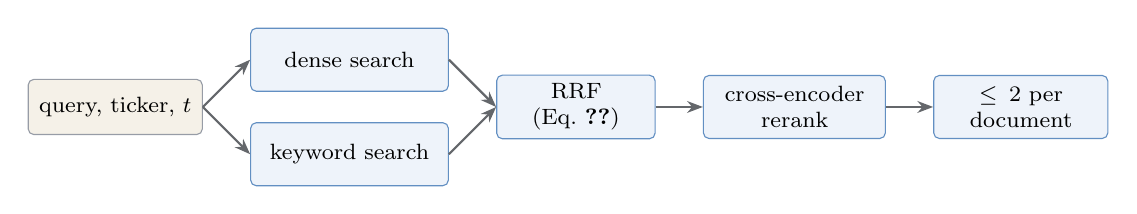
\begin{tikzpicture}[node distance=4mm and 6mm]
  \node[ext=2.0cm] (q) {query, ticker, $t$};
  \node[block=2.3cm, right=of q, yshift=6mm] (dense) {dense search};
  \node[block=2.3cm, right=of q, yshift=-6mm] (kw) {keyword search};
  \node[block=1.8cm, right=of dense, yshift=-6mm] (rrf) {RRF\\(Eq.~\ref{eq:rrf})};
  \node[block=2.1cm, right=of rrf] (rr) {cross-encoder rerank};
  \node[block=2.0cm, right=of rr] (div) {$\le 2$ per document};
  \draw[arr] (q.east) -- (dense.west);
  \draw[arr] (q.east) -- (kw.west);
  \draw[arr] (dense.east) -- (rrf.west);
  \draw[arr] (kw.east) -- (rrf.west);
  \draw[arr] (rrf) -- (rr);
  \draw[arr] (rr) -- (div);
\end{tikzpicture}
\caption{Retrieval pipeline. Both searches are restricted to documents published before $t$.}
\label{fig:retrieval}
\end{figure}

\subsection{Agent and code-enforced guardrails}
\label{sec:agent}

For each pick the agent runs a ReAct-style loop \cite{yao2022react} with four read tools (retrieval,
features, weekly prices, macro snapshot) and one write tool, \code{save\_suggestion}
(Figure~\ref{fig:agent}). A view contains a stance for a horizon (1--3 or 6--24 months) relative to SPY, a
thesis, bull and bear cases, valuation, catalysts, risks, a confidence in $[0,1]$ and its sources. Because a
4B model does not follow prompt rules reliably, the rules that matter are enforced in code at save time:

\begin{enumerate}
  \item \emph{Fixed scope.} No tool accepts a date, and the stored ticker and as-of date are set by the system.
  \item \emph{Seen citations.} Every cited identifier must have been returned by retrieval in the same session.
  \item \emph{Grounded numbers.} Every token that looks like a quantitative claim (a decimal, a percentage, a
        currency amount or a magnitude suffix) must equal, after rounding, a value returned by some tool in the
        session; a ratio such as $0.151$ may appear as $15.1\%$.
  \item \emph{Schema and language.} Required fields must be present, and text must be in English.
\end{enumerate}

\noindent A rejected save returns the reason to the model, which may correct the view. Each pick is limited
to 16 model turns and 16 tool calls, with one retry that keeps any horizon already saved, and every call is
logged.

\begin{figure}[t]
\centering
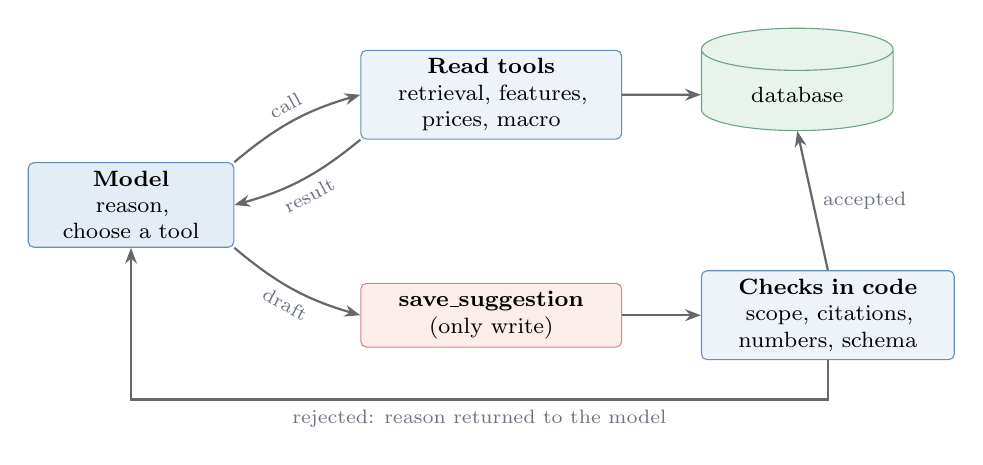
\begin{tikzpicture}[node distance=7mm and 9mm]
  \node[block=2.4cm, fill=accent!12] (llm) {\textbf{Model}\\reason, choose a tool};
  \node[block=3.1cm, right=16mm of llm, yshift=14mm] (read) {\textbf{Read tools}\\retrieval, features,\\prices, macro};
  \node[block=3.1cm, right=16mm of llm, yshift=-14mm, fill=warnfill, draw=bad!60] (save) {\textbf{save\_suggestion}\\(only write)};
  \node[block=3.0cm, right=10mm of save] (checks) {\textbf{Checks in code}\\scope, citations,\\numbers, schema};
  \node[store=2.2cm, right=10mm of read] (db) {database};
  \draw[arr] (llm.north east) to[bend left=12] node[lbl, above, sloped]{call} (read.west);
  \draw[arr] (read.south west) to[bend left=12] node[lbl, below, sloped]{result} (llm.east);
  \draw[arr] (read) -- (db);
  \draw[arr] (llm.south east) to[bend right=12] node[lbl, below, sloped]{draft} (save.west);
  \draw[arr] (save) -- (checks);
  \draw[arr] (checks.south) -- ++(0,-5mm) -| node[lbl, below, pos=0.25]{rejected: reason returned to the model} (llm.south);
  \draw[arr] (checks.north) -- node[lbl, right]{accepted} (db.south);
\end{tikzpicture}
\caption{Agent loop with save-time checks.}
\label{fig:agent}
\end{figure}

\subsection{Serverless delivery}
\label{sec:delivery}

Readers use a Flutter application published as a static site. Since a static host cannot query the
database, each pipeline run exports exactly the content the application displays into one file, encrypted
with AES-256-GCM \cite{nist80038d} under a key derived from a password with PBKDF2-SHA256 \cite{rfc8018}
($250{,}000$ iterations, random 16-byte salt, fresh 96-bit nonce per export). The application downloads the
file and decrypts it in the browser through the Web Crypto API; only the derived key is retained on the
device. The salt is kept while the password is unchanged, so devices need not re-enter it, and the file is
rewritten only when its content changes. The design trades freshness (results are as recent as the last
publication) for having no server, no domain and no running infrastructure.

% ==================================================================
\section{Experimental setup}
\label{sec:setup}

\paragraph{Hardware and software} One laptop with an NVIDIA RTX 4050 (6\,GB), 16\,GB of RAM and a 12\,GB page
file, running Windows 11; PostgreSQL 17 with pgvector in Docker; Ollama serving a text-only, 4-bit build of
Qwen3.5 4B with a 16k-token context and thinking enabled; embeddings, reranking and FinBERT on the CPU.

\paragraph{Data and run} The deployment analysed here used the screen as of 14 November 2026 (data up to the
13 November close), a two-year backfill of news and filings for the selected stocks, and one agent run on
14 November with at most 16 turns and 16 tool calls per stock and one retry. The same afternoon the
no-retrieval comparator of Section~\ref{sec:protocol} was run on the same picks and features, with the same
prompt and limits, the search tool removed and citations disabled.

\paragraph{Measurements} Screening yield; retrieval quality on a fixed ten-query set (automatic checks of
ticker, source and as-of compliance and an expected keyword in the top three, plus manual relevance
judgements by the author); guardrail activity (save attempts and rejection reasons, from the tool-call log);
properties of the stored views (citations, numeric claims, stances, confidence); and wall-clock time of each
pipeline stage.

% ==================================================================
\section{Results}
\label{sec:results}

\subsection{Screening and data}

Of 903 index members with enough price and filing history, 728 passed the quality filter and 20 were
selected (Table~\ref{tab:data}). The selection concentrated in health care (7) and energy (5), consistent
with momentum's tendency to follow recently strong sectors. The knowledge base for the twenty picks
comprised 5{,}475 documents (4{,}875 news items, 600 filings) split into 37{,}879 passages.

\begin{table}[t]
\centering\small
\caption{Screening yield and stored data after the first deployment.}
\label{tab:data}
\begin{tabular}{@{}lr@{\qquad}lr@{}}
\toprule
Screening & & Stored data & \\
\midrule
Index members screened & 903 & Daily prices & 495{,}468 \\
Passed quality filter  & 728 & XBRL facts & 429{,}924 \\
Selected               & 20  & Documents (news / filings) & 4{,}875 / 600 \\
Analysed by the agent  & 20  & Passages (chunks) & 37{,}879 \\
\bottomrule
\end{tabular}
\end{table}

\subsection{Retrieval quality}

Table~\ref{tab:retrieval} reports the ten-query evaluation. Hybrid retrieval passed every automatic check
(correct ticker and source, nothing dated at or after $t$, expected keyword in the top three) but was judged
on topic for only about seven of ten queries; the misses were queries whose answer depends on a specific
phrase (e.g.\ a product line or an export regime). Adding the cross-encoder made all ten top results on topic,
at a cost of roughly half a second per query on the CPU, so the agent reranks by default. A further five
queries about the twenty picks, run against the new database, all returned passages from the correct company.

\begin{table}[t]
\centering\small
\caption{Retrieval on the ten-query test set ($k=5$). On-topic judgements are by the author.}
\label{tab:retrieval}
\begin{tabular}{@{}lcc@{}}
\toprule
Configuration & Automatic checks passed & On-topic top results \\
\midrule
Hybrid (dense + lexical, RRF) & 10/10 & $\approx$ 7/10 \\
Hybrid + cross-encoder rerank & 10/10 & 10/10 \\
\bottomrule
\end{tabular}
\end{table}

\subsection{Guardrail activity}

The agent made 89 attempts to save a view, of which 49 (55\%) were rejected (Table~\ref{tab:guard}): 26 for a
number that matched no tool output and 23 for a missing required field. Every rejected view was later saved
in a corrected form; no stock ended without both views. Four stocks needed their retry, two after a
model-server error and two after reaching the tool-call cap. Effort varied widely across stocks
(Figure~\ref{fig:effort}), from 3 to 11 model turns in the final attempt.

\begin{table}[t]
\centering\small
\caption{Save-time guardrail activity in the first deployment (20 stocks, 2 horizons each).}
\label{tab:guard}
\begin{tabular}{@{}lr@{}}
\toprule
Measure & Value \\
\midrule
Save attempts & 89 \\
\quad rejected: number not found in any tool output & 26 \\
\quad rejected: required field missing & 23 \\
\quad accepted & 40 \\
Stocks with both views saved & 20 / 20 \\
Stocks that needed the retry & 4 \\
Tool calls (all attempts) & 253 \\
\bottomrule
\end{tabular}
\end{table}

\begin{figure}[t]
\centering
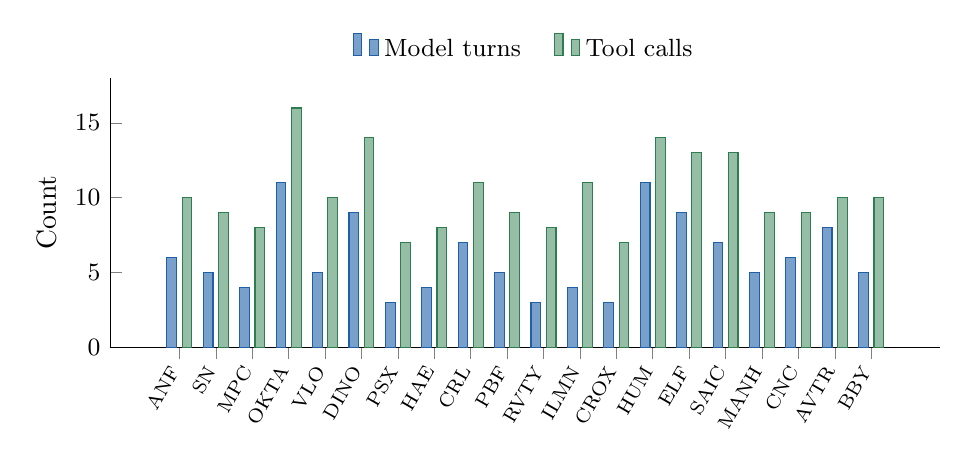
\begin{tikzpicture}
\begin{axis}[
  ybar, width=\linewidth, height=5cm, ymin=0, ymax=18, ylabel={Count},
  symbolic x coords={ANF,SN,MPC,OKTA,VLO,DINO,PSX,HAE,CRL,PBF,RVTY,ILMN,CROX,HUM,ELF,SAIC,MANH,CNC,AVTR,BBY},
  xtick=data, x tick label style={rotate=60, anchor=east, font=\scriptsize}, y tick label style={font=\small},
  bar width=3.5pt, legend columns=2, legend style={font=\small, at={(0.5,1.02)}, anchor=south, draw=none,
    /tikz/every even column/.append style={column sep=10pt}},
  axis x line*=bottom, axis y line*=left,
]
\addplot[fill=accent!60, draw=accent] coordinates {
  (ANF,6) (SN,5) (MPC,4) (OKTA,11) (VLO,5) (DINO,9) (PSX,3) (HAE,4) (CRL,7) (PBF,5)
  (RVTY,3) (ILMN,4) (CROX,3) (HUM,11) (ELF,9) (SAIC,7) (MANH,5) (CNC,6) (AVTR,8) (BBY,5)};
\addplot[fill=good!50, draw=good] coordinates {
  (ANF,10) (SN,9) (MPC,8) (OKTA,16) (VLO,10) (DINO,14) (PSX,7) (HAE,8) (CRL,11) (PBF,9)
  (RVTY,8) (ILMN,11) (CROX,7) (HUM,14) (ELF,13) (SAIC,13) (MANH,9) (CNC,9) (AVTR,10) (BBY,10)};
\legend{Model turns, Tool calls}
\end{axis}
\end{tikzpicture}
\caption{Agent effort per stock in the final attempt, in screen rank order.}
\label{fig:effort}
\end{figure}

\subsection{Properties of the stored views}

The 40 views averaged 228 words and 3.8 citations each (minimum 3, maximum 6), drawing on 130 distinct
passages from 120 documents (73 passages from filings, 57 from news). They contained 470 numeric claims
(11.8 per view), all of which matched a tool output at save time. Stances were mostly bullish, more so at the
short horizon (Figure~\ref{fig:stances}); stated confidence lay between 0.55 and 0.62 (mean 0.59).

\begin{figure}[t]
\centering
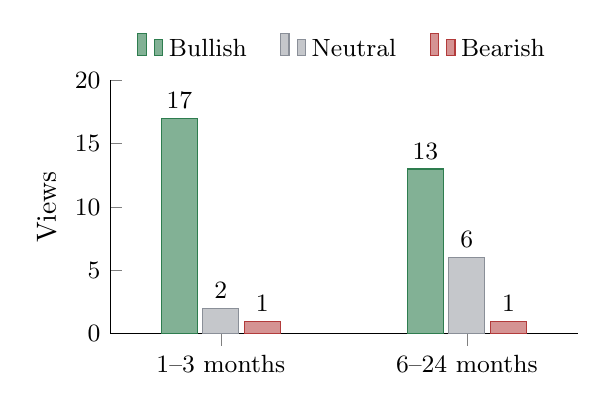
\begin{tikzpicture}
\begin{axis}[
  ybar, width=0.62\linewidth, height=4.8cm, ymin=0, ymax=20, ylabel={Views},
  symbolic x coords={1--3 months, 6--24 months}, xtick=data, enlarge x limits=0.45,
  bar width=13pt, nodes near coords, nodes near coords style={font=\small},
  legend style={font=\small, at={(0.5,1.03)}, anchor=south, legend columns=3, draw=none,
    /tikz/every even column/.append style={column sep=10pt}},
  axis x line*=bottom, axis y line*=left, x tick label style={font=\small}, y tick label style={font=\small},
]
\addplot[fill=good!60, draw=good] coordinates {(1--3 months,17) (6--24 months,13)};
\addplot[fill=neutral!50, draw=neutral] coordinates {(1--3 months,2) (6--24 months,6)};
\addplot[fill=bad!55, draw=bad] coordinates {(1--3 months,1) (6--24 months,1)};
\legend{Bullish, Neutral, Bearish}
\end{axis}
\end{tikzpicture}
\caption{Stance distribution of the 40 views, relative to SPY.}
\label{fig:stances}
\end{figure}

\subsection{Retrieval ablation in the first week}
\label{sec:ablation}

Table~\ref{tab:ablation} compares the full system with the no-retrieval variant. Both completed every
stock. Without documents the model was slightly less bullish at the short horizon and agreed with the full
system on 13 of 20 stances at each horizon. Chance-corrected agreement was low over one to three months
($\kappa = 0.07$) and fair over six to twenty-four months ($\kappa = 0.32$), so retrieved evidence changes
short-horizon calls more than long-horizon ones. Agreement says nothing about accuracy, which the protocol
measures once outcomes close.

\begin{table}[t]
\centering\small
\caption{The full system and the no-retrieval variant on the same twenty picks, week of 14 November 2026.}
\label{tab:ablation}
\begin{tabular}{@{}lrr@{}}
\toprule
 & Full & No retrieval \\
\midrule
Run status, views saved & ok, 40 & ok, 40 \\
Wall-clock time & 32 min & 31 min \\
Save attempts rejected & 49 of 89 & 73 of 113 \\
\quad of which unmatched numbers & 26 & 71 \\
\quad of which period labels only (``3m'') & 13 & 51 \\
\quad of which missing or invalid fields & 23 & 2 \\
Citations & 152 & 0 \\
1--3 months: bullish / neutral / bearish & 17 / 2 / 1 & 14 / 6 / 0 \\
6--24 months: bullish / neutral / bearish & 13 / 6 / 1 & 12 / 6 / 2 \\
Mean confidence & 0.59 & 0.59 \\
\midrule
Same stance, 1--3 months & \multicolumn{2}{c}{13 of 20, $\kappa = 0.07$} \\
Same stance, 6--24 months & \multicolumn{2}{c}{13 of 20, $\kappa = 0.32$} \\
\bottomrule
\end{tabular}
\end{table}

The rejection log also exposed a false positive in the number check. A token such as ``3m'' is parsed as
three million, which no tool output contains, although the model means three months (``3m momentum'').
Such rejections made up half of the unmatched-number refusals in the full run and almost three quarters in
the ablation, where the model leans more on momentum features. They cost model turns but no views: three
stocks needed a second attempt in the ablation and none were lost. After the first week the check was
amended: a whole number of at most 60 written directly against ``m'' with no currency sign is read as a
period in months. Amounts such as ``\$3m'', ``3.5m'' or ``250m'' are still checked as millions.

\subsection{Efficiency}

Table~\ref{tab:time} gives wall-clock times. Generation dominates the weekly cost at about 96 seconds per
stock. Incremental ingestion keeps the daily refresh short: on the second refresh of the day, prices for 21
tickers amounted to 126 new rows rather than roughly 11{,}000, and the whole refresh took under a minute. The
encrypted export of everything the application shows was 607\,KB.

\begin{table}[t]
\centering\small
\caption{Wall-clock time per stage in the first deployment.}
\label{tab:time}
\begin{tabular}{@{}lrl@{}}
\toprule
Stage & Time & Volume \\
\midrule
Screen: index lists, prices, SEC facts, ranking & 9.6 min & 903 stocks \\
Backfill of news and filings for the picks & 6.3 min & 20 stocks \\
Chunking and embedding (CPU) & 12.7 min & 5{,}474 documents \\
News sentiment (CPU) & 5.2 min & 4{,}874 items \\
Agent run (GPU) & 32 min & 20 stocks, 40 views \\
Daily incremental refresh & 57 s & 21 tickers \\
\bottomrule
\end{tabular}
\end{table}

% ==================================================================
\section{Discussion}
\label{sec:discussion}

\paragraph{What the guardrails buy} The most informative number in the deployment is the rejection rate.
More than half of the model's attempts to save were refused, and 26 of those refusals concerned numbers that
no tool had produced. Each would otherwise have been a plausible, specific and unsupported figure in a
published view. The model corrected every rejected view when told why, which suggests that a small model is
usable for this task when correctness is enforced outside it rather than requested in the prompt.

\paragraph{Bullish skew} Thirty of forty views were bullish. Two explanations overlap: the screen selects
stocks with strong recent momentum, so continued outperformance is the default narrative, and language models
tend towards agreeable conclusions. Separating the two requires the baselines in Section~\ref{sec:protocol}.

\paragraph{What retrieval changes} The ablation suggests that documents mainly move the short-horizon view,
where news and recent filings are most relevant, while the long-horizon view is largely set by the features
both variants share. Whether that movement is towards or away from the outcome is the question the paired
comparison in Section~\ref{sec:protocol} is designed to answer.

\paragraph{Narrow confidence} Confidence values clustered between 0.55 and 0.62, as the prompt requests
caution. Whether these values are calibrated \cite{guo2017calibration} is an empirical question; a constant
would be uninformative even if well calibrated on average.

\paragraph{Operational lessons} The failures in the first deployment were environmental rather than
algorithmic: memory exhaustion while loading the embedding model, a single very large filing, and the model
server holding about 6\,GB after the run. Each led to a code change (streamed downloads with a size cap,
stopping rather than marking documents failed on out-of-memory errors, and unloading the model at the end of
a run). On consumer hardware, resource management is part of correctness.

% ==================================================================
\section{Limitations and threats to validity}
\label{sec:limitations}

\begin{itemize}
  \item \emph{No outcome evaluation yet.} The results describe behaviour and grounding, not predictive value.
  \item \emph{One deployment.} All agent statistics come from a single week: one full run and one
        no-retrieval run on the same 20 stocks.
  \item \emph{Small, author-labelled retrieval set.} Ten queries with relevance judged by the author; no
        inter-annotator agreement.
  \item \emph{Grounding is lexical.} The number check verifies that a value appeared in a tool output, not that
        it is attributed to the right quantity; a correct number under a wrong label passes. It also
        erred the other way: period labels such as ``3m'' were read as millions and rejected
        (Section~\ref{sec:ablation}). The correction took effect from the second week, so the first week
        ran under a stricter check than later weeks; we report this as a protocol amendment, and the
        evaluation can be repeated without week one.
  \item \emph{Residual look-ahead.} Inputs are point-in-time, but the model's training data may contain later
        information \cite{glasserman2023assessing}; backtests before its training cutoff are optimistic.
  \item \emph{Survivorship.} The universe is current index membership.
  \item \emph{Data coverage.} Free news covers about one year and only headlines and summaries; filings are
        truncated at 300{,}000 characters.
\end{itemize}

% ==================================================================
\section{Pre-specified evaluation protocol}
\label{sec:protocol}

To separate the contribution of the agent from that of the screen, every weekly run will be scored once its
horizons have elapsed, against four comparators: (i) the screen alone (all picks treated as bullish);
(ii) a random sample of quality-passing stocks; (iii) the agent without retrieval (features only); and (iv) the
full system. For each view we will record the excess return over SPY at 21, 63 and 252 trading days, and
report:

\begin{itemize}
  \item hit rate of the stance against the sign of the excess return, with a binomial test against 50\%
        (neutral views have no direction and are excluded from hit rates);
  \item mean excess return of bullish minus bearish views, with block-bootstrap confidence intervals over weeks;
  \item calibration of the stated confidence (Brier score and reliability diagram) \cite{guo2017calibration};
  \item citation faithfulness: the share of claims supported by their cited passage, judged on a stratified
        sample by two annotators, with Cohen's $\kappa$.
\end{itemize}

\noindent The primary analysis uses the 63-trading-day horizon and requires at least twelve weekly runs
(240 stocks, 480 views). Results will be reported whether or not they favour the system.

The protocol is implemented in the released code and runs after every weekly screen. Each (view, horizon)
pair is scored once, when its window has closed: entry is the first trading day on or after the view's
as-of date, and returns use adjusted closes. The random comparator is seeded by the screen date so that it
can be reproduced, and the no-retrieval comparator is generated by the same agent with the search tool
removed and citations disabled; it is stored alongside the full system's views but never published. At the
time of writing one week of both variants had been recorded and no window had closed: all 120 (view, horizon)
pairs of the full system, the corresponding no-retrieval pairs and 2{,}304 baseline pairs were still open.
The first 21-day windows close in mid-December 2026 and the primary analysis becomes possible after twelve
weeks have closed at 63 trading days, around May 2027.

% ==================================================================
\section{Conclusion}
\label{sec:conclusion}

TI Agent shows that a 4-billion-parameter model on consumer hardware can produce structured, cited equity
research when the surrounding system fixes the scope, supplies every number, checks every citation and
refuses unsupported output. In its first deployment the checks rejected more than half of the model's save
attempts and the model corrected all of them, yielding 40 views whose 470 numbers and 152 citations can each be
traced to a computed value or a retrieved passage. Whether these views carry information about future returns
is the subject of the protocol in Section~\ref{sec:protocol}. Future work also includes portfolio
construction from the views, including a comparison of classical optimisation with QAOA
\cite{farhi2014quantum, brandhofer2022benchmarking}.

% ==================================================================
\section*{Ethics and disclaimer}
TI Agent is a research system. Its output is not investment advice and it does not trade. Views are
published only to readers who hold the password, and this paper reports aggregate statistics rather than
recommendations for individual securities.

\section*{Data and code availability}
The source code is available at \url{https://github.com/nsskn982/TI-Agent}. Market and news data are not
redistributed because of the providers' terms; SEC filings and FRED series are public and can be
retrieved with the provided code.

\section*{Declaration of competing interest}
The author declares no competing interests.

\section*{Funding}
This research received no specific grant from any funding agency.

\section*{CRediT authorship contribution statement}
\textbf{Nanda Srikanth Saroj Kumar Nanda:} Conceptualization, Methodology, Software, Investigation, Writing
-- original draft, Writing -- review \& editing.

\section*{Declaration of generative AI and AI-assisted technologies in the writing process}
% Edit this statement so that it describes exactly how AI tools were used.
During the preparation of this work the author used Claude (Anthropic) to assist with software development,
data analysis and drafting of the manuscript. After using this tool, the author reviewed and edited the
content as needed and takes full responsibility for the content of the publication.

\bibliographystyle{elsarticle-num}
\bibliography{../report/references}

\end{document}
